\section*{Directed Acyclic Graphs}

Let $G = (V, E)$ be a directed graph. 
If a vertex $v\in V$ does not have any in-edges~(i.e., \emph{in-degree} is 0), we call it \emph{source vertex};
if a vertex $v\in V$ does not have any out-edges~(i.e., \emph{out-degree} is 0), we call it \emph{sink vertex}.

A directed graph may contain multiple source vertices or sink vertices,
or may not have any source vertex or sink vertex. (Can you give such examples?)

\begin{claim}
A DAG $G=(V,E)$ always has source vertex and sink vertex.
\end{claim}
\emph{Proof.} Let's prove it by contradiction. Assume that $G$ does not contain any source.
First, $G$ must not contain self-loop as otherwise $G$ won't be a DAG.
Let $v$ be any vertex in $V$. As $v$ is not a source, we know that there exists some vertex $u$ points to $v$, i.e., $(u,v)\in E$.
Now since $u$ is not a source then there must exist another vertex $w$ such that $(w,u)\in E$.
Notice that $w \neq v$ as otherwise there will be a cycle: $v = w \to u \to v$.
This means that $w$ is a new vertex. Again as $w$ is not a source, there must exist another \emph{new} vertex points to it.
This process can be extended infinitely following the fact and assumption that $G$ is a DAG and all vertices not are sources,
but this is not possible as the number of vertices is limited. 
The existence of sink can be proved symmetrically. \qed


Following above fact, we can design an algorithm to find a linearization of a DAG: it iteratively
finds source vertex and removes it and its adjacent edges.

\begin{minipage}{0.8\textwidth}
	\aaA {7}{Algorithm find-linearization ($G = (V, E)$)}\xxx
	\aab {init $X$ as empty list;}\xxx
	\aaB {4}{while ($|X| < |V|$)}\xxx
	\aac {arbitrarily find a source vertex $u$ of $G$;}\xxx
	\aac {add $u$ to the end of $X$;}\xxx
	\aac {remove $u$ and its adjacent edges;}\xxx
	\aab {end while;}\xxx
	\aaa {end algorithm;}\xxx
\end{minipage}

This algorithm is correct. First, when a vertex $u$ is added to $X$,
it is a source vertex of the current graph, which means that
$\{w\mid (w, u)\in E\}$ is either empty or all of them
have been added to $X$. Second, $X$ will include all vertices.
This is because, a source always exists in a DAG~(as we just proved).
The above algorithm is more a framework, as how we update the graph
is not given specifically, and which affects the running time.

Above algorithm also gives a constructive proof that, a DAG can always
be linearized. This completes the proof stated in previous lecture: a directed graph is a DAG if and only if it can be linearized.

\begin{claim}
Let $X$ be any linearization of a DAG. Then the first vertex of $X$ is a source vertex and 
the last vertex of of $X$ is a sink vertex.
\label{claim:source}
\end{claim}

\emph{Proof.} Let $v_1$ be the first vertex of $X$. Suppose that $v_1$ is not a source of $X$. 
By definition of (not being a) source vertex, there exists $(u,v_1)\in E$. Then by the definition
of linearization, we know that $u$ will be before $v_1$ in $X$, contradicting to the fact that
$v_1$ is the first element of $X$.
The other side can be proved symmetrically. \qed

We can use above algorithm to constructively prove following statement.

\begin{claim}
Let $G = (V, E)$ be a DAG. A vertex $u\in V$ is a source if and only if 
there exists a linearization $X$ of $G$ such that $u$ is the first vertex in $X$.
\end{claim}

\emph{Proof.} We first prove that, if $u$ is a source, then there exists a linearization
where $u$ is the first vertex of $X$. We prove it by showing that,
we can construct such a linearization $X$. We can use above algorithm,
and in its first step, we simply pick $u$. The correctness of above algorithm
explains the rest.  The other side is exactly Claim~\ref{claim:source}, which we have proved. \qed

\section*{Connectivity of Directed Graphs}

For a directed graph $G = (V,E)$, its structure of connectivity can be represented as a new
directed graph, called \emph{meta-graph}, denoted as $G_M = (V_M, E_M)$.
Each of the vertices of the meta-graph corresponds to a connected component of $G$,
and two vertices $C_i, C_j  \in V_M$ are connected by edge $(C_i, C_j) \in E_M$
if and only if there exists edge $(u,v)\in E$ such that $u\in C_i$ and $v\in C_j$.
An example of meta-graph is given below.

\begin{figure}[h!]
\centering{

\tikzset{every picture/.style={line width=0.75pt}} %set default line width to 0.75pt        

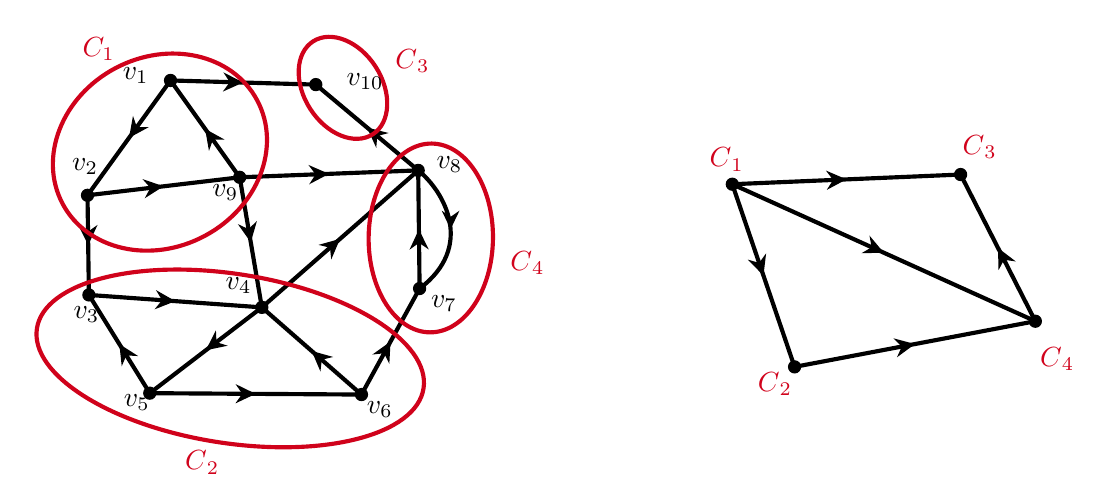
\begin{tikzpicture}[x=0.5pt,y=0.5pt,yscale=-1,xscale=1]
%uncomment if require: \path (0,510); %set diagram left start at 0, and has height of 510

%Flowchart: Connector [id:dp5937668531638635] 
\draw  [fill={rgb, 255:red, 0; green, 0; blue, 0 }  ,fill opacity=1 ] (139,106) .. controls (139,103.58) and (140.96,101.62) .. (143.38,101.62) .. controls (145.79,101.62) and (147.75,103.58) .. (147.75,106) .. controls (147.75,108.42) and (145.79,110.38) .. (143.38,110.38) .. controls (140.96,110.38) and (139,108.42) .. (139,106) -- cycle ;
%Flowchart: Connector [id:dp6657935561963445] 
\draw  [fill={rgb, 255:red, 0; green, 0; blue, 0 }  ,fill opacity=1 ] (244,109) .. controls (244,106.58) and (245.96,104.62) .. (248.38,104.62) .. controls (250.79,104.62) and (252.75,106.58) .. (252.75,109) .. controls (252.75,111.42) and (250.79,113.38) .. (248.38,113.38) .. controls (245.96,113.38) and (244,111.42) .. (244,109) -- cycle ;
%Flowchart: Connector [id:dp14354113795738999] 
\draw  [fill={rgb, 255:red, 0; green, 0; blue, 0 }  ,fill opacity=1 ] (124,332) .. controls (124,329.58) and (125.96,327.62) .. (128.38,327.62) .. controls (130.79,327.62) and (132.75,329.58) .. (132.75,332) .. controls (132.75,334.42) and (130.79,336.38) .. (128.38,336.38) .. controls (125.96,336.38) and (124,334.42) .. (124,332) -- cycle ;
%Flowchart: Connector [id:dp3081556962622095] 
\draw  [fill={rgb, 255:red, 0; green, 0; blue, 0 }  ,fill opacity=1 ] (79,189) .. controls (79,186.58) and (80.96,184.62) .. (83.38,184.62) .. controls (85.79,184.62) and (87.75,186.58) .. (87.75,189) .. controls (87.75,191.42) and (85.79,193.38) .. (83.38,193.38) .. controls (80.96,193.38) and (79,191.42) .. (79,189) -- cycle ;
%Flowchart: Connector [id:dp20013554043379078] 
\draw  [fill={rgb, 255:red, 0; green, 0; blue, 0 }  ,fill opacity=1 ] (189,176) .. controls (189,173.58) and (190.96,171.62) .. (193.38,171.62) .. controls (195.79,171.62) and (197.75,173.58) .. (197.75,176) .. controls (197.75,178.42) and (195.79,180.38) .. (193.38,180.38) .. controls (190.96,180.38) and (189,178.42) .. (189,176) -- cycle ;
%Straight Lines [id:da8865551056781525] 
\draw [color={rgb, 255:red, 0; green, 0; blue, 0 }  ,draw opacity=1 ][line width=1.5]    (83.38,189) -- (143.38,106) ;
\draw [shift={(113.38,147.5)}, rotate = 305.86] [fill={rgb, 255:red, 0; green, 0; blue, 0 }  ,fill opacity=1 ][line width=0.08]  [draw opacity=0] (14.56,-6.99) -- (0,0) -- (14.56,6.99) -- (9.67,0) -- cycle    ;
%Straight Lines [id:da4408247919919335] 
\draw [color={rgb, 255:red, 0; green, 0; blue, 0 }  ,draw opacity=1 ][line width=1.5]    (128.38,332) -- (209.38,270) ;
\draw [shift={(168.88,301)}, rotate = 322.57] [fill={rgb, 255:red, 0; green, 0; blue, 0 }  ,fill opacity=1 ][line width=0.08]  [draw opacity=0] (14.56,-6.99) -- (0,0) -- (14.56,6.99) -- (9.67,0) -- cycle    ;
%Straight Lines [id:da8012008000621113] 
\draw [color={rgb, 255:red, 0; green, 0; blue, 0 }  ,draw opacity=1 ][line width=1.5]    (193.38,176) -- (83.38,189) ;
\draw [shift={(138.38,182.5)}, rotate = 173.26] [fill={rgb, 255:red, 0; green, 0; blue, 0 }  ,fill opacity=1 ][line width=0.08]  [draw opacity=0] (14.56,-6.99) -- (0,0) -- (14.56,6.99) -- (9.67,0) -- cycle    ;
%Straight Lines [id:da01269837290493725] 
\draw [color={rgb, 255:red, 0; green, 0; blue, 0 }  ,draw opacity=1 ][line width=1.5]    (128.38,332) -- (84.38,261) ;
\draw [shift={(106.38,296.5)}, rotate = 418.21000000000004] [fill={rgb, 255:red, 0; green, 0; blue, 0 }  ,fill opacity=1 ][line width=0.08]  [draw opacity=0] (14.56,-6.99) -- (0,0) -- (14.56,6.99) -- (9.67,0) -- cycle    ;
%Flowchart: Connector [id:dp01738972677326256] 
\draw  [fill={rgb, 255:red, 0; green, 0; blue, 0 }  ,fill opacity=1 ] (277,333) .. controls (277,330.58) and (278.96,328.62) .. (281.38,328.62) .. controls (283.79,328.62) and (285.75,330.58) .. (285.75,333) .. controls (285.75,335.42) and (283.79,337.38) .. (281.38,337.38) .. controls (278.96,337.38) and (277,335.42) .. (277,333) -- cycle ;
%Straight Lines [id:da9151099863353562] 
\draw [color={rgb, 255:red, 0; green, 0; blue, 0 }  ,draw opacity=1 ][line width=1.5]    (281.38,333) -- (323.38,256.38) ;
\draw [shift={(302.38,294.69)}, rotate = 478.73] [fill={rgb, 255:red, 0; green, 0; blue, 0 }  ,fill opacity=1 ][line width=0.08]  [draw opacity=0] (14.56,-6.99) -- (0,0) -- (14.56,6.99) -- (9.67,0) -- cycle    ;
%Straight Lines [id:da8589700496158776] 
\draw [color={rgb, 255:red, 0; green, 0; blue, 0 }  ,draw opacity=1 ][line width=1.5]    (128.38,332) -- (281.38,333) ;
\draw [shift={(204.88,332.5)}, rotate = 180.37] [fill={rgb, 255:red, 0; green, 0; blue, 0 }  ,fill opacity=1 ][line width=0.08]  [draw opacity=0] (14.56,-6.99) -- (0,0) -- (14.56,6.99) -- (9.67,0) -- cycle    ;
%Flowchart: Connector [id:dp23564521467293476] 
\draw  [fill={rgb, 255:red, 0; green, 0; blue, 0 }  ,fill opacity=1 ] (319,256.38) .. controls (319,253.96) and (320.96,252) .. (323.38,252) .. controls (325.79,252) and (327.75,253.96) .. (327.75,256.38) .. controls (327.75,258.79) and (325.79,260.75) .. (323.38,260.75) .. controls (320.96,260.75) and (319,258.79) .. (319,256.38) -- cycle ;
%Straight Lines [id:da5765902383361479] 
\draw [color={rgb, 255:red, 0; green, 0; blue, 0 }  ,draw opacity=1 ][line width=1.5]    (323.38,256.38) -- (322.38,171) ;
\draw [shift={(322.88,213.69)}, rotate = 449.33] [fill={rgb, 255:red, 0; green, 0; blue, 0 }  ,fill opacity=1 ][line width=0.08]  [draw opacity=0] (14.56,-6.99) -- (0,0) -- (14.56,6.99) -- (9.67,0) -- cycle    ;
%Straight Lines [id:da6859280233883376] 
\draw [color={rgb, 255:red, 0; green, 0; blue, 0 }  ,draw opacity=1 ][line width=1.5]    (322.38,171) -- (248.38,109) ;
\draw [shift={(285.38,140)}, rotate = 399.96000000000004] [fill={rgb, 255:red, 0; green, 0; blue, 0 }  ,fill opacity=1 ][line width=0.08]  [draw opacity=0] (14.56,-6.99) -- (0,0) -- (14.56,6.99) -- (9.67,0) -- cycle    ;
%Straight Lines [id:da329141247373788] 
\draw [color={rgb, 255:red, 0; green, 0; blue, 0 }  ,draw opacity=1 ][line width=1.5]    (143.38,106) -- (193.38,176) ;
\draw [shift={(168.38,141)}, rotate = 54.46] [fill={rgb, 255:red, 0; green, 0; blue, 0 }  ,fill opacity=1 ][line width=0.08]  [draw opacity=0] (14.56,-6.99) -- (0,0) -- (14.56,6.99) -- (9.67,0) -- cycle    ;
%Straight Lines [id:da25009890870323437] 
\draw [color={rgb, 255:red, 0; green, 0; blue, 0 }  ,draw opacity=1 ][line width=1.5]    (209.38,270) -- (281.38,333) ;
\draw [shift={(245.38,301.5)}, rotate = 41.19] [fill={rgb, 255:red, 0; green, 0; blue, 0 }  ,fill opacity=1 ][line width=0.08]  [draw opacity=0] (14.56,-6.99) -- (0,0) -- (14.56,6.99) -- (9.67,0) -- cycle    ;
%Flowchart: Connector [id:dp20561620581532858] 
\draw  [fill={rgb, 255:red, 0; green, 0; blue, 0 }  ,fill opacity=1 ] (205,270) .. controls (205,267.58) and (206.96,265.62) .. (209.38,265.62) .. controls (211.79,265.62) and (213.75,267.58) .. (213.75,270) .. controls (213.75,272.42) and (211.79,274.38) .. (209.38,274.38) .. controls (206.96,274.38) and (205,272.42) .. (205,270) -- cycle ;
%Flowchart: Connector [id:dp4014605163661533] 
\draw  [fill={rgb, 255:red, 0; green, 0; blue, 0 }  ,fill opacity=1 ] (80,261) .. controls (80,258.58) and (81.96,256.62) .. (84.38,256.62) .. controls (86.79,256.62) and (88.75,258.58) .. (88.75,261) .. controls (88.75,263.42) and (86.79,265.38) .. (84.38,265.38) .. controls (81.96,265.38) and (80,263.42) .. (80,261) -- cycle ;
%Flowchart: Connector [id:dp14845565107772662] 
\draw  [fill={rgb, 255:red, 0; green, 0; blue, 0 }  ,fill opacity=1 ] (318,171) .. controls (318,168.58) and (319.96,166.62) .. (322.38,166.62) .. controls (324.79,166.62) and (326.75,168.58) .. (326.75,171) .. controls (326.75,173.42) and (324.79,175.38) .. (322.38,175.38) .. controls (319.96,175.38) and (318,173.42) .. (318,171) -- cycle ;
%Straight Lines [id:da3881378688310262] 
\draw [color={rgb, 255:red, 0; green, 0; blue, 0 }  ,draw opacity=1 ][line width=1.5]    (209.38,270) -- (84.38,261) ;
\draw [shift={(146.88,265.5)}, rotate = 184.12] [fill={rgb, 255:red, 0; green, 0; blue, 0 }  ,fill opacity=1 ][line width=0.08]  [draw opacity=0] (14.56,-6.99) -- (0,0) -- (14.56,6.99) -- (9.67,0) -- cycle    ;
%Curve Lines [id:da8015709651805362] 
\draw [line width=1.5]    (323.38,256.38) .. controls (363.38,226.38) and (341.68,186.52) .. (322.38,171) ;
\draw [shift={(345.77,213.48)}, rotate = 270.05] [fill={rgb, 255:red, 0; green, 0; blue, 0 }  ][line width=0.08]  [draw opacity=0] (13.4,-6.43) -- (0,0) -- (13.4,6.44) -- (8.9,0) -- cycle    ;
%Straight Lines [id:da4386825484478063] 
\draw [color={rgb, 255:red, 0; green, 0; blue, 0 }  ,draw opacity=1 ][line width=1.5]    (209.38,270) -- (322.38,171) ;
\draw [shift={(265.88,220.5)}, rotate = 498.78] [fill={rgb, 255:red, 0; green, 0; blue, 0 }  ,fill opacity=1 ][line width=0.08]  [draw opacity=0] (14.56,-6.99) -- (0,0) -- (14.56,6.99) -- (9.67,0) -- cycle    ;
%Straight Lines [id:da26616639892534444] 
\draw [color={rgb, 255:red, 0; green, 0; blue, 0 }  ,draw opacity=1 ][line width=1.5]    (193.38,176) -- (209.38,270) ;
\draw [shift={(201.38,223)}, rotate = 260.34000000000003] [fill={rgb, 255:red, 0; green, 0; blue, 0 }  ,fill opacity=1 ][line width=0.08]  [draw opacity=0] (14.56,-6.99) -- (0,0) -- (14.56,6.99) -- (9.67,0) -- cycle    ;
%Straight Lines [id:da34500416847135773] 
\draw [color={rgb, 255:red, 0; green, 0; blue, 0 }  ,draw opacity=1 ][line width=1.5]    (83.38,189) -- (84.38,261) ;
\draw [shift={(83.88,225)}, rotate = 269.2] [fill={rgb, 255:red, 0; green, 0; blue, 0 }  ,fill opacity=1 ][line width=0.08]  [draw opacity=0] (14.56,-6.99) -- (0,0) -- (14.56,6.99) -- (9.67,0) -- cycle    ;
%Straight Lines [id:da4267721016610234] 
\draw [color={rgb, 255:red, 0; green, 0; blue, 0 }  ,draw opacity=1 ][line width=1.5]    (193.38,176) -- (322.38,171) ;
\draw [shift={(257.88,173.5)}, rotate = 537.78] [fill={rgb, 255:red, 0; green, 0; blue, 0 }  ,fill opacity=1 ][line width=0.08]  [draw opacity=0] (14.56,-6.99) -- (0,0) -- (14.56,6.99) -- (9.67,0) -- cycle    ;
%Straight Lines [id:da8164594223234878] 
\draw [color={rgb, 255:red, 0; green, 0; blue, 0 }  ,draw opacity=1 ][line width=1.5]    (143.38,106) -- (248.38,109) ;
\draw [shift={(195.88,107.5)}, rotate = 181.64] [fill={rgb, 255:red, 0; green, 0; blue, 0 }  ,fill opacity=1 ][line width=0.08]  [draw opacity=0] (14.56,-6.99) -- (0,0) -- (14.56,6.99) -- (9.67,0) -- cycle    ;
%Shape: Ellipse [id:dp27109176732345586] 
\draw  [color={rgb, 255:red, 208; green, 2; blue, 27 }  ,draw opacity=1 ][line width=1.5]  (65.39,195.12) .. controls (47.61,161.62) and (64.68,117.75) .. (103.52,97.13) .. controls (142.37,76.52) and (188.27,86.96) .. (206.05,120.45) .. controls (223.83,153.95) and (206.76,197.82) .. (167.91,218.44) .. controls (129.07,239.06) and (83.17,228.61) .. (65.39,195.12) -- cycle ;
%Shape: Ellipse [id:dp0877469193537469] 
\draw  [color={rgb, 255:red, 208; green, 2; blue, 27 }  ,draw opacity=1 ][line width=1.5]  (46.82,285.18) .. controls (52.01,251.81) and (118.75,234.47) .. (195.91,246.46) .. controls (273.06,258.44) and (331.4,295.21) .. (326.22,328.58) .. controls (321.04,361.95) and (254.29,379.29) .. (177.14,367.3) .. controls (99.98,355.32) and (41.64,318.55) .. (46.82,285.18) -- cycle ;
%Shape: Ellipse [id:dp6318272598845582] 
\draw  [color={rgb, 255:red, 208; green, 2; blue, 27 }  ,draw opacity=1 ][line width=1.5]  (332.2,151.61) .. controls (357.02,151.88) and (376.8,182.63) .. (376.4,220.31) .. controls (376,257.98) and (355.56,288.31) .. (330.75,288.04) .. controls (305.94,287.78) and (286.15,257.02) .. (286.55,219.35) .. controls (286.96,181.68) and (307.39,151.35) .. (332.2,151.61) -- cycle ;
%Shape: Ellipse [id:dp1869855316402914] 
\draw  [color={rgb, 255:red, 208; green, 2; blue, 27 }  ,draw opacity=1 ][line width=1.5]  (246.45,77.74) .. controls (259.53,69.36) and (279.77,77.6) .. (291.66,96.15) .. controls (303.55,114.71) and (302.58,136.54) .. (289.5,144.92) .. controls (276.42,153.3) and (256.19,145.05) .. (244.3,126.5) .. controls (232.41,107.95) and (233.38,86.12) .. (246.45,77.74) -- cycle ;
%Flowchart: Connector [id:dp51888588365958] 
\draw  [fill={rgb, 255:red, 0; green, 0; blue, 0 }  ,fill opacity=1 ] (590,313) .. controls (590,310.58) and (591.96,308.62) .. (594.38,308.62) .. controls (596.79,308.62) and (598.75,310.58) .. (598.75,313) .. controls (598.75,315.42) and (596.79,317.38) .. (594.38,317.38) .. controls (591.96,317.38) and (590,315.42) .. (590,313) -- cycle ;
%Straight Lines [id:da6410921260405182] 
\draw [color={rgb, 255:red, 0; green, 0; blue, 0 }  ,draw opacity=1 ][line width=1.5]    (768.38,280) -- (549.38,181) ;
\draw [shift={(658.88,230.5)}, rotate = 204.33] [fill={rgb, 255:red, 0; green, 0; blue, 0 }  ,fill opacity=1 ][line width=0.08]  [draw opacity=0] (14.56,-6.99) -- (0,0) -- (14.56,6.99) -- (9.67,0) -- cycle    ;
%Straight Lines [id:da8627356399127929] 
\draw [color={rgb, 255:red, 0; green, 0; blue, 0 }  ,draw opacity=1 ][line width=1.5]    (768.38,280) -- (714.38,174) ;
\draw [shift={(741.38,227)}, rotate = 423] [fill={rgb, 255:red, 0; green, 0; blue, 0 }  ,fill opacity=1 ][line width=0.08]  [draw opacity=0] (14.56,-6.99) -- (0,0) -- (14.56,6.99) -- (9.67,0) -- cycle    ;
%Flowchart: Connector [id:dp5660576336850748] 
\draw  [fill={rgb, 255:red, 0; green, 0; blue, 0 }  ,fill opacity=1 ] (710,174) .. controls (710,171.58) and (711.96,169.62) .. (714.38,169.62) .. controls (716.79,169.62) and (718.75,171.58) .. (718.75,174) .. controls (718.75,176.42) and (716.79,178.38) .. (714.38,178.38) .. controls (711.96,178.38) and (710,176.42) .. (710,174) -- cycle ;
%Flowchart: Connector [id:dp5784688617216504] 
\draw  [fill={rgb, 255:red, 0; green, 0; blue, 0 }  ,fill opacity=1 ] (545,181) .. controls (545,178.58) and (546.96,176.62) .. (549.38,176.62) .. controls (551.79,176.62) and (553.75,178.58) .. (553.75,181) .. controls (553.75,183.42) and (551.79,185.38) .. (549.38,185.38) .. controls (546.96,185.38) and (545,183.42) .. (545,181) -- cycle ;
%Straight Lines [id:da35390930720516367] 
\draw [color={rgb, 255:red, 0; green, 0; blue, 0 }  ,draw opacity=1 ][line width=1.5]    (594.38,313) -- (549.38,181) ;
\draw [shift={(571.88,247)}, rotate = 251.18] [fill={rgb, 255:red, 0; green, 0; blue, 0 }  ,fill opacity=1 ][line width=0.08]  [draw opacity=0] (14.56,-6.99) -- (0,0) -- (14.56,6.99) -- (9.67,0) -- cycle    ;
%Straight Lines [id:da16486738526478106] 
\draw [color={rgb, 255:red, 0; green, 0; blue, 0 }  ,draw opacity=1 ][line width=1.5]    (549.38,181) -- (714.38,174) ;
\draw [shift={(631.88,177.5)}, rotate = 537.5699999999999] [fill={rgb, 255:red, 0; green, 0; blue, 0 }  ,fill opacity=1 ][line width=0.08]  [draw opacity=0] (14.56,-6.99) -- (0,0) -- (14.56,6.99) -- (9.67,0) -- cycle    ;
%Flowchart: Connector [id:dp49963370359380055] 
\draw  [fill={rgb, 255:red, 0; green, 0; blue, 0 }  ,fill opacity=1 ] (764,280) .. controls (764,277.58) and (765.96,275.62) .. (768.38,275.62) .. controls (770.79,275.62) and (772.75,277.58) .. (772.75,280) .. controls (772.75,282.42) and (770.79,284.38) .. (768.38,284.38) .. controls (765.96,284.38) and (764,282.42) .. (764,280) -- cycle ;
%Straight Lines [id:da8408093021248022] 
\draw [color={rgb, 255:red, 0; green, 0; blue, 0 }  ,draw opacity=1 ][line width=1.5]    (768.38,280) -- (594.38,313) ;
\draw [shift={(681.38,296.5)}, rotate = 169.26] [fill={rgb, 255:red, 0; green, 0; blue, 0 }  ,fill opacity=1 ][line width=0.08]  [draw opacity=0] (14.56,-6.99) -- (0,0) -- (14.56,6.99) -- (9.67,0) -- cycle    ;

% Text Node
\draw (107,94.93) node [anchor=north west][inner sep=0.75pt]   [align=left] {$\displaystyle v_{1}$};
% Text Node
\draw (71.38,267.31) node [anchor=north west][inner sep=0.75pt]   [align=left] {$\displaystyle v_{3}$};
% Text Node
\draw (107.75,330.93) node [anchor=north west][inner sep=0.75pt]   [align=left] {$\displaystyle v_{5}$};
% Text Node
\draw (181.38,246.31) node [anchor=north west][inner sep=0.75pt]   [align=left] {$\displaystyle v_{4}$};
% Text Node
\draw (70.38,160.31) node [anchor=north west][inner sep=0.75pt]   [align=left] {$\displaystyle v_{2}$};
% Text Node
\draw (171.75,179.29) node [anchor=north west][inner sep=0.75pt]   [align=left] {$\displaystyle v_{9}$};
% Text Node
\draw (329.75,259.31) node [anchor=north west][inner sep=0.75pt]   [align=left] {$\displaystyle v_{7}$};
% Text Node
\draw (283.38,335.93) node [anchor=north west][inner sep=0.75pt]   [align=left] {$\displaystyle v_{6}$};
% Text Node
\draw (333.75,159.29) node [anchor=north west][inner sep=0.75pt]   [align=left] {$\displaystyle v_{8}$};
% Text Node
\draw (268.75,99.29) node [anchor=north west][inner sep=0.75pt]   [align=left] {$\displaystyle v_{10}$};
% Text Node
\draw (78,72.93) node [anchor=north west][inner sep=0.75pt]   [align=left] {$\displaystyle \textcolor[rgb]{0.82,0.01,0.11}{C_{1}}$};
% Text Node
\draw (152,371.93) node [anchor=north west][inner sep=0.75pt]   [align=left] {$\displaystyle \textcolor[rgb]{0.82,0.01,0.11}{C}\textcolor[rgb]{0.82,0.01,0.11}{_{2}}$};
% Text Node
\draw (387,227.93) node [anchor=north west][inner sep=0.75pt]   [align=left] {$\displaystyle \textcolor[rgb]{0.82,0.01,0.11}{C}\textcolor[rgb]{0.82,0.01,0.11}{_{4}}$};
% Text Node
\draw (304,81.93) node [anchor=north west][inner sep=0.75pt]   [align=left] {$\displaystyle \textcolor[rgb]{0.82,0.01,0.11}{C}\textcolor[rgb]{0.82,0.01,0.11}{_{3}}$};
% Text Node
\draw (566,314.93) node [anchor=north west][inner sep=0.75pt]   [align=left] {$\displaystyle \textcolor[rgb]{0.82,0.01,0.11}{C}\textcolor[rgb]{0.82,0.01,0.11}{_{2}}$};
% Text Node
\draw (770,296.93) node [anchor=north west][inner sep=0.75pt]   [align=left] {$\displaystyle \textcolor[rgb]{0.82,0.01,0.11}{C}\textcolor[rgb]{0.82,0.01,0.11}{_{4}}$};
% Text Node
\draw (531,152.93) node [anchor=north west][inner sep=0.75pt]   [align=left] {$\displaystyle \textcolor[rgb]{0.82,0.01,0.11}{C}\textcolor[rgb]{0.82,0.01,0.11}{_{1}}$};
% Text Node
\draw (714,143.93) node [anchor=north west][inner sep=0.75pt]   [align=left] {$\displaystyle \textcolor[rgb]{0.82,0.01,0.11}{C}\textcolor[rgb]{0.82,0.01,0.11}{_{3}}$};


\end{tikzpicture}

}
\caption{Example of meta-graph.}
\label{fig:meta-graph}
\end{figure}

Meta-graph has an important property: it does not contain cycles, i.e., it is a directed acyclic graph~(DAG).

\begin{claim}
The meta-graph $G_M$ of any directed graph $G$ is a directed acyclic graph.
\end{claim}

\emph{Proof.} Suppose conversely that $G_M$ contains a cycle, $C_1 \to C_2 \to C_k \to C_1$,
then the union of the vertices in these connected components form a single connected component,
contradicting to the \emph{maximal} property of connected component. \qed

We now design algorithms to determine the connected components of directed graphs and then to construct
the corresponding meta-graph.
Recall that the DFS algorithm introduced in Lecture A9 can successfully determine all connected components in an undirected graph.
Does this work also work for directed graph? Let's try. See Figure~\ref{fig:dfs-meta}.
Recall that the (top-layer) of the DFS algorithm is to tranverse all vertices in some ordering,
and if the current vertex $v$ is not yet visited, we will explore $v$.
For the example in Figure~\ref{fig:dfs-meta}, let's try it with the (natrual) ordering $v_1, v_2, \cdots, v_{10}$.
The resulting visited array is given in the figure~(please make sure you try it yourself).
Unfortunately, it does not give all connected components. In fact, the vertices marked as ``1''s are the union of $C_3$ and $C_4$,
and the vertices marked as ``2''s are the union of $C_1$ and $C_2$.
The reason is quite clear: we start with explore $v_1$, and during it all vertices reachable from $v_1$ will be marked as ``1'' in the visted array.
It turns out that $v_1$ is in connected component $C_4$, and $C_4$ can reach $C_3$ in the meta-graph.
Therefore, all vertices in $C_4$ and $C_3$ are reachable from $v_1$; consequently, the visited array is set as ``1'' for 
vertices in $C_4$ and $C_3$ during explore $v_1$. 
Similarly, we can also see why the vertices marked as ``2''s are the union of $C_1$ and $C_2$.
After exploring $v_1$, $\{v_1,v_2,v_7\}$ are visited; the next unvisited vertex is $v_3$ according to above natural ordering,
the the algorithm will explore $v_3$.
Again, during it all (unvisited) vertices reachable from $v_3$ will be marked as ``2'' in the visted array.
It turns out that $v_3$ is in connected component $C_1$, and $C_1$ can reach $C_2$ in the meta-graph.
Therefore, all vertices in $C_1$ and $C_2$ are reachable from $v_2$;
consequently, the visited array is set as ``2'' for 
vertices in $C_1$ and $C_2$. 


\begin{figure}[h!]
\centering{

\tikzset{every picture/.style={line width=0.75pt}} %set default line width to 0.75pt        

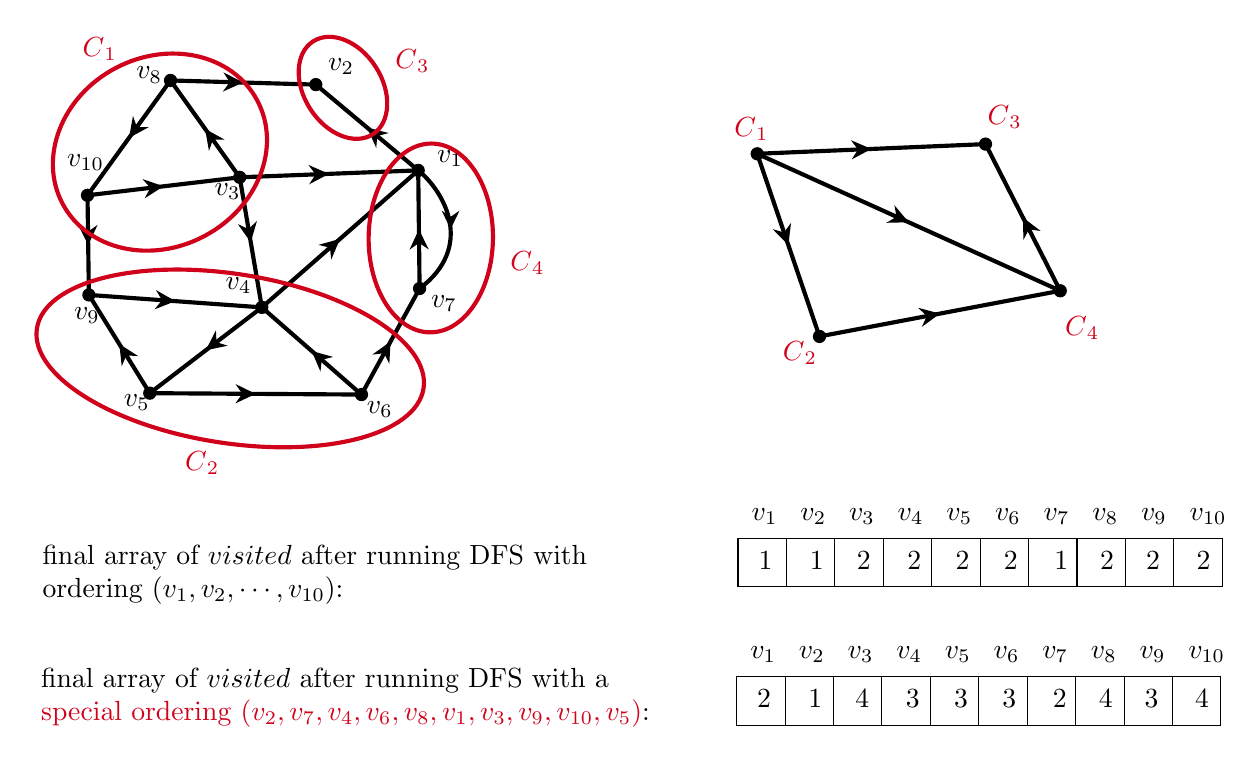
\begin{tikzpicture}[x=0.5pt,y=0.5pt,yscale=-1,xscale=1]
%uncomment if require: \path (0,553); %set diagram left start at 0, and has height of 553

%Flowchart: Connector [id:dp33314190657915177] 
\draw  [fill={rgb, 255:red, 0; green, 0; blue, 0 }  ,fill opacity=1 ] (137,52) .. controls (137,49.58) and (138.96,47.62) .. (141.38,47.62) .. controls (143.79,47.62) and (145.75,49.58) .. (145.75,52) .. controls (145.75,54.42) and (143.79,56.38) .. (141.38,56.38) .. controls (138.96,56.38) and (137,54.42) .. (137,52) -- cycle ;
%Flowchart: Connector [id:dp9493779383807376] 
\draw  [fill={rgb, 255:red, 0; green, 0; blue, 0 }  ,fill opacity=1 ] (242,55) .. controls (242,52.58) and (243.96,50.62) .. (246.38,50.62) .. controls (248.79,50.62) and (250.75,52.58) .. (250.75,55) .. controls (250.75,57.42) and (248.79,59.38) .. (246.38,59.38) .. controls (243.96,59.38) and (242,57.42) .. (242,55) -- cycle ;
%Flowchart: Connector [id:dp6669453073289408] 
\draw  [fill={rgb, 255:red, 0; green, 0; blue, 0 }  ,fill opacity=1 ] (122,278) .. controls (122,275.58) and (123.96,273.62) .. (126.38,273.62) .. controls (128.79,273.62) and (130.75,275.58) .. (130.75,278) .. controls (130.75,280.42) and (128.79,282.38) .. (126.38,282.38) .. controls (123.96,282.38) and (122,280.42) .. (122,278) -- cycle ;
%Flowchart: Connector [id:dp333713085025936] 
\draw  [fill={rgb, 255:red, 0; green, 0; blue, 0 }  ,fill opacity=1 ] (77,135) .. controls (77,132.58) and (78.96,130.62) .. (81.38,130.62) .. controls (83.79,130.62) and (85.75,132.58) .. (85.75,135) .. controls (85.75,137.42) and (83.79,139.38) .. (81.38,139.38) .. controls (78.96,139.38) and (77,137.42) .. (77,135) -- cycle ;
%Flowchart: Connector [id:dp9629725454572109] 
\draw  [fill={rgb, 255:red, 0; green, 0; blue, 0 }  ,fill opacity=1 ] (187,122) .. controls (187,119.58) and (188.96,117.62) .. (191.38,117.62) .. controls (193.79,117.62) and (195.75,119.58) .. (195.75,122) .. controls (195.75,124.42) and (193.79,126.38) .. (191.38,126.38) .. controls (188.96,126.38) and (187,124.42) .. (187,122) -- cycle ;
%Straight Lines [id:da6590518201146447] 
\draw [color={rgb, 255:red, 0; green, 0; blue, 0 }  ,draw opacity=1 ][line width=1.5]    (81.38,135) -- (141.38,52) ;
\draw [shift={(111.38,93.5)}, rotate = 305.86] [fill={rgb, 255:red, 0; green, 0; blue, 0 }  ,fill opacity=1 ][line width=0.08]  [draw opacity=0] (14.56,-6.99) -- (0,0) -- (14.56,6.99) -- (9.67,0) -- cycle    ;
%Straight Lines [id:da1177530387710749] 
\draw [color={rgb, 255:red, 0; green, 0; blue, 0 }  ,draw opacity=1 ][line width=1.5]    (126.38,278) -- (207.38,216) ;
\draw [shift={(166.88,247)}, rotate = 322.57] [fill={rgb, 255:red, 0; green, 0; blue, 0 }  ,fill opacity=1 ][line width=0.08]  [draw opacity=0] (14.56,-6.99) -- (0,0) -- (14.56,6.99) -- (9.67,0) -- cycle    ;
%Straight Lines [id:da8328235451162237] 
\draw [color={rgb, 255:red, 0; green, 0; blue, 0 }  ,draw opacity=1 ][line width=1.5]    (191.38,122) -- (81.38,135) ;
\draw [shift={(136.38,128.5)}, rotate = 173.26] [fill={rgb, 255:red, 0; green, 0; blue, 0 }  ,fill opacity=1 ][line width=0.08]  [draw opacity=0] (14.56,-6.99) -- (0,0) -- (14.56,6.99) -- (9.67,0) -- cycle    ;
%Straight Lines [id:da13491976799128524] 
\draw [color={rgb, 255:red, 0; green, 0; blue, 0 }  ,draw opacity=1 ][line width=1.5]    (126.38,278) -- (82.38,207) ;
\draw [shift={(104.38,242.5)}, rotate = 58.21] [fill={rgb, 255:red, 0; green, 0; blue, 0 }  ,fill opacity=1 ][line width=0.08]  [draw opacity=0] (14.56,-6.99) -- (0,0) -- (14.56,6.99) -- (9.67,0) -- cycle    ;
%Flowchart: Connector [id:dp015404259848177726] 
\draw  [fill={rgb, 255:red, 0; green, 0; blue, 0 }  ,fill opacity=1 ] (275,279) .. controls (275,276.58) and (276.96,274.62) .. (279.38,274.62) .. controls (281.79,274.62) and (283.75,276.58) .. (283.75,279) .. controls (283.75,281.42) and (281.79,283.38) .. (279.38,283.38) .. controls (276.96,283.38) and (275,281.42) .. (275,279) -- cycle ;
%Straight Lines [id:da9050593875476026] 
\draw [color={rgb, 255:red, 0; green, 0; blue, 0 }  ,draw opacity=1 ][line width=1.5]    (279.38,279) -- (321.38,202.38) ;
\draw [shift={(300.38,240.69)}, rotate = 118.73] [fill={rgb, 255:red, 0; green, 0; blue, 0 }  ,fill opacity=1 ][line width=0.08]  [draw opacity=0] (14.56,-6.99) -- (0,0) -- (14.56,6.99) -- (9.67,0) -- cycle    ;
%Straight Lines [id:da6930328339194429] 
\draw [color={rgb, 255:red, 0; green, 0; blue, 0 }  ,draw opacity=1 ][line width=1.5]    (126.38,278) -- (279.38,279) ;
\draw [shift={(202.88,278.5)}, rotate = 180.37] [fill={rgb, 255:red, 0; green, 0; blue, 0 }  ,fill opacity=1 ][line width=0.08]  [draw opacity=0] (14.56,-6.99) -- (0,0) -- (14.56,6.99) -- (9.67,0) -- cycle    ;
%Flowchart: Connector [id:dp8561555389036362] 
\draw  [fill={rgb, 255:red, 0; green, 0; blue, 0 }  ,fill opacity=1 ] (317,202.38) .. controls (317,199.96) and (318.96,198) .. (321.38,198) .. controls (323.79,198) and (325.75,199.96) .. (325.75,202.38) .. controls (325.75,204.79) and (323.79,206.75) .. (321.38,206.75) .. controls (318.96,206.75) and (317,204.79) .. (317,202.38) -- cycle ;
%Straight Lines [id:da4194772983165912] 
\draw [color={rgb, 255:red, 0; green, 0; blue, 0 }  ,draw opacity=1 ][line width=1.5]    (321.38,202.38) -- (320.38,117) ;
\draw [shift={(320.88,159.69)}, rotate = 89.33] [fill={rgb, 255:red, 0; green, 0; blue, 0 }  ,fill opacity=1 ][line width=0.08]  [draw opacity=0] (14.56,-6.99) -- (0,0) -- (14.56,6.99) -- (9.67,0) -- cycle    ;
%Straight Lines [id:da26627336015658065] 
\draw [color={rgb, 255:red, 0; green, 0; blue, 0 }  ,draw opacity=1 ][line width=1.5]    (320.38,117) -- (246.38,55) ;
\draw [shift={(283.38,86)}, rotate = 39.96] [fill={rgb, 255:red, 0; green, 0; blue, 0 }  ,fill opacity=1 ][line width=0.08]  [draw opacity=0] (14.56,-6.99) -- (0,0) -- (14.56,6.99) -- (9.67,0) -- cycle    ;
%Straight Lines [id:da6540321478063363] 
\draw [color={rgb, 255:red, 0; green, 0; blue, 0 }  ,draw opacity=1 ][line width=1.5]    (141.38,52) -- (191.38,122) ;
\draw [shift={(166.38,87)}, rotate = 54.46] [fill={rgb, 255:red, 0; green, 0; blue, 0 }  ,fill opacity=1 ][line width=0.08]  [draw opacity=0] (14.56,-6.99) -- (0,0) -- (14.56,6.99) -- (9.67,0) -- cycle    ;
%Straight Lines [id:da980763773394733] 
\draw [color={rgb, 255:red, 0; green, 0; blue, 0 }  ,draw opacity=1 ][line width=1.5]    (207.38,216) -- (279.38,279) ;
\draw [shift={(243.38,247.5)}, rotate = 41.19] [fill={rgb, 255:red, 0; green, 0; blue, 0 }  ,fill opacity=1 ][line width=0.08]  [draw opacity=0] (14.56,-6.99) -- (0,0) -- (14.56,6.99) -- (9.67,0) -- cycle    ;
%Flowchart: Connector [id:dp884579398191617] 
\draw  [fill={rgb, 255:red, 0; green, 0; blue, 0 }  ,fill opacity=1 ] (203,216) .. controls (203,213.58) and (204.96,211.62) .. (207.38,211.62) .. controls (209.79,211.62) and (211.75,213.58) .. (211.75,216) .. controls (211.75,218.42) and (209.79,220.38) .. (207.38,220.38) .. controls (204.96,220.38) and (203,218.42) .. (203,216) -- cycle ;
%Flowchart: Connector [id:dp3352413725395753] 
\draw  [fill={rgb, 255:red, 0; green, 0; blue, 0 }  ,fill opacity=1 ] (78,207) .. controls (78,204.58) and (79.96,202.62) .. (82.38,202.62) .. controls (84.79,202.62) and (86.75,204.58) .. (86.75,207) .. controls (86.75,209.42) and (84.79,211.38) .. (82.38,211.38) .. controls (79.96,211.38) and (78,209.42) .. (78,207) -- cycle ;
%Flowchart: Connector [id:dp01230167588576514] 
\draw  [fill={rgb, 255:red, 0; green, 0; blue, 0 }  ,fill opacity=1 ] (316,117) .. controls (316,114.58) and (317.96,112.62) .. (320.38,112.62) .. controls (322.79,112.62) and (324.75,114.58) .. (324.75,117) .. controls (324.75,119.42) and (322.79,121.38) .. (320.38,121.38) .. controls (317.96,121.38) and (316,119.42) .. (316,117) -- cycle ;
%Straight Lines [id:da2185567480823013] 
\draw [color={rgb, 255:red, 0; green, 0; blue, 0 }  ,draw opacity=1 ][line width=1.5]    (207.38,216) -- (82.38,207) ;
\draw [shift={(144.88,211.5)}, rotate = 184.12] [fill={rgb, 255:red, 0; green, 0; blue, 0 }  ,fill opacity=1 ][line width=0.08]  [draw opacity=0] (14.56,-6.99) -- (0,0) -- (14.56,6.99) -- (9.67,0) -- cycle    ;
%Curve Lines [id:da3916533808212287] 
\draw [line width=1.5]    (321.38,202.38) .. controls (361.38,172.38) and (339.68,132.52) .. (320.38,117) ;
\draw [shift={(343.77,159.48)}, rotate = 270.05] [fill={rgb, 255:red, 0; green, 0; blue, 0 }  ][line width=0.08]  [draw opacity=0] (13.4,-6.43) -- (0,0) -- (13.4,6.44) -- (8.9,0) -- cycle    ;
%Straight Lines [id:da9071388879776039] 
\draw [color={rgb, 255:red, 0; green, 0; blue, 0 }  ,draw opacity=1 ][line width=1.5]    (207.38,216) -- (320.38,117) ;
\draw [shift={(263.88,166.5)}, rotate = 138.78] [fill={rgb, 255:red, 0; green, 0; blue, 0 }  ,fill opacity=1 ][line width=0.08]  [draw opacity=0] (14.56,-6.99) -- (0,0) -- (14.56,6.99) -- (9.67,0) -- cycle    ;
%Straight Lines [id:da17399207464778044] 
\draw [color={rgb, 255:red, 0; green, 0; blue, 0 }  ,draw opacity=1 ][line width=1.5]    (191.38,122) -- (207.38,216) ;
\draw [shift={(199.38,169)}, rotate = 260.34] [fill={rgb, 255:red, 0; green, 0; blue, 0 }  ,fill opacity=1 ][line width=0.08]  [draw opacity=0] (14.56,-6.99) -- (0,0) -- (14.56,6.99) -- (9.67,0) -- cycle    ;
%Straight Lines [id:da8016859457087312] 
\draw [color={rgb, 255:red, 0; green, 0; blue, 0 }  ,draw opacity=1 ][line width=1.5]    (81.38,135) -- (82.38,207) ;
\draw [shift={(81.88,171)}, rotate = 269.2] [fill={rgb, 255:red, 0; green, 0; blue, 0 }  ,fill opacity=1 ][line width=0.08]  [draw opacity=0] (14.56,-6.99) -- (0,0) -- (14.56,6.99) -- (9.67,0) -- cycle    ;
%Straight Lines [id:da8138783684306082] 
\draw [color={rgb, 255:red, 0; green, 0; blue, 0 }  ,draw opacity=1 ][line width=1.5]    (191.38,122) -- (320.38,117) ;
\draw [shift={(255.88,119.5)}, rotate = 177.78] [fill={rgb, 255:red, 0; green, 0; blue, 0 }  ,fill opacity=1 ][line width=0.08]  [draw opacity=0] (14.56,-6.99) -- (0,0) -- (14.56,6.99) -- (9.67,0) -- cycle    ;
%Straight Lines [id:da24392431611835252] 
\draw [color={rgb, 255:red, 0; green, 0; blue, 0 }  ,draw opacity=1 ][line width=1.5]    (141.38,52) -- (246.38,55) ;
\draw [shift={(193.88,53.5)}, rotate = 181.64] [fill={rgb, 255:red, 0; green, 0; blue, 0 }  ,fill opacity=1 ][line width=0.08]  [draw opacity=0] (14.56,-6.99) -- (0,0) -- (14.56,6.99) -- (9.67,0) -- cycle    ;
%Shape: Ellipse [id:dp837267975011143] 
\draw  [color={rgb, 255:red, 208; green, 2; blue, 27 }  ,draw opacity=1 ][line width=1.5]  (63.39,141.12) .. controls (45.61,107.62) and (62.68,63.75) .. (101.52,43.13) .. controls (140.37,22.52) and (186.27,32.96) .. (204.05,66.45) .. controls (221.83,99.95) and (204.76,143.82) .. (165.91,164.44) .. controls (127.07,185.06) and (81.17,174.61) .. (63.39,141.12) -- cycle ;
%Shape: Ellipse [id:dp6301102730017264] 
\draw  [color={rgb, 255:red, 208; green, 2; blue, 27 }  ,draw opacity=1 ][line width=1.5]  (44.82,231.18) .. controls (50.01,197.81) and (116.75,180.47) .. (193.91,192.46) .. controls (271.06,204.44) and (329.4,241.21) .. (324.22,274.58) .. controls (319.04,307.95) and (252.29,325.29) .. (175.14,313.3) .. controls (97.98,301.32) and (39.64,264.55) .. (44.82,231.18) -- cycle ;
%Shape: Ellipse [id:dp9534249176688527] 
\draw  [color={rgb, 255:red, 208; green, 2; blue, 27 }  ,draw opacity=1 ][line width=1.5]  (330.2,97.61) .. controls (355.02,97.88) and (374.8,128.63) .. (374.4,166.31) .. controls (374,203.98) and (353.56,234.31) .. (328.75,234.04) .. controls (303.94,233.78) and (284.15,203.02) .. (284.55,165.35) .. controls (284.96,127.68) and (305.39,97.35) .. (330.2,97.61) -- cycle ;
%Shape: Ellipse [id:dp8449632734349601] 
\draw  [color={rgb, 255:red, 208; green, 2; blue, 27 }  ,draw opacity=1 ][line width=1.5]  (244.45,23.74) .. controls (257.53,15.36) and (277.77,23.6) .. (289.66,42.15) .. controls (301.55,60.71) and (300.58,82.54) .. (287.5,90.92) .. controls (274.42,99.3) and (254.19,91.05) .. (242.3,72.5) .. controls (230.41,53.95) and (231.38,32.12) .. (244.45,23.74) -- cycle ;
%Flowchart: Connector [id:dp603695290762529] 
\draw  [fill={rgb, 255:red, 0; green, 0; blue, 0 }  ,fill opacity=1 ] (606,237) .. controls (606,234.58) and (607.96,232.62) .. (610.38,232.62) .. controls (612.79,232.62) and (614.75,234.58) .. (614.75,237) .. controls (614.75,239.42) and (612.79,241.38) .. (610.38,241.38) .. controls (607.96,241.38) and (606,239.42) .. (606,237) -- cycle ;
%Straight Lines [id:da27444933364712354] 
\draw [color={rgb, 255:red, 0; green, 0; blue, 0 }  ,draw opacity=1 ][line width=1.5]    (784.38,204) -- (565.38,105) ;
\draw [shift={(674.88,154.5)}, rotate = 204.33] [fill={rgb, 255:red, 0; green, 0; blue, 0 }  ,fill opacity=1 ][line width=0.08]  [draw opacity=0] (14.56,-6.99) -- (0,0) -- (14.56,6.99) -- (9.67,0) -- cycle    ;
%Straight Lines [id:da6238918789957093] 
\draw [color={rgb, 255:red, 0; green, 0; blue, 0 }  ,draw opacity=1 ][line width=1.5]    (784.38,204) -- (730.38,98) ;
\draw [shift={(757.38,151)}, rotate = 63] [fill={rgb, 255:red, 0; green, 0; blue, 0 }  ,fill opacity=1 ][line width=0.08]  [draw opacity=0] (14.56,-6.99) -- (0,0) -- (14.56,6.99) -- (9.67,0) -- cycle    ;
%Flowchart: Connector [id:dp07658274147850641] 
\draw  [fill={rgb, 255:red, 0; green, 0; blue, 0 }  ,fill opacity=1 ] (726,98) .. controls (726,95.58) and (727.96,93.62) .. (730.38,93.62) .. controls (732.79,93.62) and (734.75,95.58) .. (734.75,98) .. controls (734.75,100.42) and (732.79,102.38) .. (730.38,102.38) .. controls (727.96,102.38) and (726,100.42) .. (726,98) -- cycle ;
%Flowchart: Connector [id:dp6792415791877835] 
\draw  [fill={rgb, 255:red, 0; green, 0; blue, 0 }  ,fill opacity=1 ] (561,105) .. controls (561,102.58) and (562.96,100.62) .. (565.38,100.62) .. controls (567.79,100.62) and (569.75,102.58) .. (569.75,105) .. controls (569.75,107.42) and (567.79,109.38) .. (565.38,109.38) .. controls (562.96,109.38) and (561,107.42) .. (561,105) -- cycle ;
%Straight Lines [id:da6954252151831065] 
\draw [color={rgb, 255:red, 0; green, 0; blue, 0 }  ,draw opacity=1 ][line width=1.5]    (610.38,237) -- (565.38,105) ;
\draw [shift={(587.88,171)}, rotate = 251.18] [fill={rgb, 255:red, 0; green, 0; blue, 0 }  ,fill opacity=1 ][line width=0.08]  [draw opacity=0] (14.56,-6.99) -- (0,0) -- (14.56,6.99) -- (9.67,0) -- cycle    ;
%Straight Lines [id:da21094314981608042] 
\draw [color={rgb, 255:red, 0; green, 0; blue, 0 }  ,draw opacity=1 ][line width=1.5]    (565.38,105) -- (730.38,98) ;
\draw [shift={(647.88,101.5)}, rotate = 177.57] [fill={rgb, 255:red, 0; green, 0; blue, 0 }  ,fill opacity=1 ][line width=0.08]  [draw opacity=0] (14.56,-6.99) -- (0,0) -- (14.56,6.99) -- (9.67,0) -- cycle    ;
%Flowchart: Connector [id:dp8786817451944372] 
\draw  [fill={rgb, 255:red, 0; green, 0; blue, 0 }  ,fill opacity=1 ] (780,204) .. controls (780,201.58) and (781.96,199.62) .. (784.38,199.62) .. controls (786.79,199.62) and (788.75,201.58) .. (788.75,204) .. controls (788.75,206.42) and (786.79,208.38) .. (784.38,208.38) .. controls (781.96,208.38) and (780,206.42) .. (780,204) -- cycle ;
%Straight Lines [id:da6613494332963039] 
\draw [color={rgb, 255:red, 0; green, 0; blue, 0 }  ,draw opacity=1 ][line width=1.5]    (784.38,204) -- (610.38,237) ;
\draw [shift={(697.38,220.5)}, rotate = 169.26] [fill={rgb, 255:red, 0; green, 0; blue, 0 }  ,fill opacity=1 ][line width=0.08]  [draw opacity=0] (14.56,-6.99) -- (0,0) -- (14.56,6.99) -- (9.67,0) -- cycle    ;
%Shape: Grid [id:dp7216183755073775] 
\draw  [draw opacity=0] (551.5,382.87) -- (901.5,382.87) -- (901.5,417.87) -- (551.5,417.87) -- cycle ; \draw   (586.5,382.87) -- (586.5,417.87)(621.5,382.87) -- (621.5,417.87)(656.5,382.87) -- (656.5,417.87)(691.5,382.87) -- (691.5,417.87)(726.5,382.87) -- (726.5,417.87)(761.5,382.87) -- (761.5,417.87)(796.5,382.87) -- (796.5,417.87)(831.5,382.87) -- (831.5,417.87)(866.5,382.87) -- (866.5,417.87) ; \draw    ; \draw   (551.5,382.87) -- (901.5,382.87) -- (901.5,417.87) -- (551.5,417.87) -- cycle ;
%Shape: Grid [id:dp08811438988655107] 
\draw  [draw opacity=0] (550.5,482.87) -- (900.5,482.87) -- (900.5,517.87) -- (550.5,517.87) -- cycle ; \draw   (585.5,482.87) -- (585.5,517.87)(620.5,482.87) -- (620.5,517.87)(655.5,482.87) -- (655.5,517.87)(690.5,482.87) -- (690.5,517.87)(725.5,482.87) -- (725.5,517.87)(760.5,482.87) -- (760.5,517.87)(795.5,482.87) -- (795.5,517.87)(830.5,482.87) -- (830.5,517.87)(865.5,482.87) -- (865.5,517.87) ; \draw    ; \draw   (550.5,482.87) -- (900.5,482.87) -- (900.5,517.87) -- (550.5,517.87) -- cycle ;

% Text Node
\draw (332.2,100.61) node [anchor=north west][inner sep=0.75pt]   [align=left] {$\displaystyle v_{1}$};
% Text Node
\draw (171.38,124.38) node [anchor=north west][inner sep=0.75pt]   [align=left] {$\displaystyle v_{3}$};
% Text Node
\draw (105.75,277) node [anchor=north west][inner sep=0.75pt]   [align=left] {$\displaystyle v_{5}$};
% Text Node
\draw (179.38,192.38) node [anchor=north west][inner sep=0.75pt]   [align=left] {$\displaystyle v_{4}$};
% Text Node
\draw (253.38,34.38) node [anchor=north west][inner sep=0.75pt]   [align=left] {$\displaystyle v_{2}$};
% Text Node
\draw (69.75,214.35) node [anchor=north west][inner sep=0.75pt]   [align=left] {$\displaystyle v_{9}$};
% Text Node
\draw (327.75,205.38) node [anchor=north west][inner sep=0.75pt]   [align=left] {$\displaystyle v_{7}$};
% Text Node
\draw (281.38,282) node [anchor=north west][inner sep=0.75pt]   [align=left] {$\displaystyle v_{6}$};
% Text Node
\draw (114.75,40.35) node [anchor=north west][inner sep=0.75pt]   [align=left] {$\displaystyle v_{8}$};
% Text Node
\draw (64.75,103.35) node [anchor=north west][inner sep=0.75pt]   [align=left] {$\displaystyle v_{10}$};
% Text Node
\draw (76,19) node [anchor=north west][inner sep=0.75pt]   [align=left] {$\displaystyle \textcolor[rgb]{0.82,0.01,0.11}{C}\textcolor[rgb]{0.82,0.01,0.11}{_{1}}$};
% Text Node
\draw (150,318) node [anchor=north west][inner sep=0.75pt]   [align=left] {$\displaystyle \textcolor[rgb]{0.82,0.01,0.11}{C}\textcolor[rgb]{0.82,0.01,0.11}{_{2}}$};
% Text Node
\draw (385,174) node [anchor=north west][inner sep=0.75pt]   [align=left] {$\displaystyle \textcolor[rgb]{0.82,0.01,0.11}{C}\textcolor[rgb]{0.82,0.01,0.11}{_{4}}$};
% Text Node
\draw (302,28) node [anchor=north west][inner sep=0.75pt]   [align=left] {$\displaystyle \textcolor[rgb]{0.82,0.01,0.11}{C}\textcolor[rgb]{0.82,0.01,0.11}{_{3}}$};
% Text Node
\draw (582,239) node [anchor=north west][inner sep=0.75pt]   [align=left] {$\displaystyle \textcolor[rgb]{0.82,0.01,0.11}{C}\textcolor[rgb]{0.82,0.01,0.11}{_{2}}$};
% Text Node
\draw (786,221) node [anchor=north west][inner sep=0.75pt]   [align=left] {$\displaystyle \textcolor[rgb]{0.82,0.01,0.11}{C}\textcolor[rgb]{0.82,0.01,0.11}{_{4}}$};
% Text Node
\draw (547,77) node [anchor=north west][inner sep=0.75pt]   [align=left] {$\displaystyle \textcolor[rgb]{0.82,0.01,0.11}{C}\textcolor[rgb]{0.82,0.01,0.11}{_{1}}$};
% Text Node
\draw (730,68) node [anchor=north west][inner sep=0.75pt]   [align=left] {$\displaystyle \textcolor[rgb]{0.82,0.01,0.11}{C}\textcolor[rgb]{0.82,0.01,0.11}{_{3}}$};
% Text Node
\draw (47,385.93) node [anchor=north west][inner sep=0.75pt]   [align=left] {final array of $\displaystyle visited$ after running DFS with\\ordering $\displaystyle ( v_{1} ,v_{2} ,\cdots ,v_{10})$:};
% Text Node
\draw (672,390.37) node [anchor=north west][inner sep=0.75pt]   [align=left] {$\displaystyle 2$};
% Text Node
\draw (706.83,390.37) node [anchor=north west][inner sep=0.75pt]   [align=left] {$\displaystyle 2$};
% Text Node
\draw (741.66,390.37) node [anchor=north west][inner sep=0.75pt]   [align=left] {$\displaystyle 2$};
% Text Node
\draw (844.49,390.37) node [anchor=north west][inner sep=0.75pt]   [align=left] {$\displaystyle 2$};
% Text Node
\draw (811.32,390.37) node [anchor=north west][inner sep=0.75pt]   [align=left] {$\displaystyle 2$};
% Text Node
\draw (778.15,390.37) node [anchor=north west][inner sep=0.75pt]   [align=left] {$\displaystyle 1$};
% Text Node
\draw (881,390.37) node [anchor=north west][inner sep=0.75pt]   [align=left] {$\displaystyle 2$};
% Text Node
\draw (564.49,390.37) node [anchor=north west][inner sep=0.75pt]   [align=left] {$\displaystyle 1$};
% Text Node
\draw (601.49,390.37) node [anchor=north west][inner sep=0.75pt]   [align=left] {$\displaystyle 1$};
% Text Node
\draw (635.49,390.37) node [anchor=north west][inner sep=0.75pt]   [align=left] {$\displaystyle 2$};
% Text Node
\draw (665,359.37) node [anchor=north west][inner sep=0.75pt]   [align=left] {$\displaystyle v_{4}$};
% Text Node
\draw (700.17,359.37) node [anchor=north west][inner sep=0.75pt]   [align=left] {$\displaystyle v_{5}$};
% Text Node
\draw (735.34,359.37) node [anchor=north west][inner sep=0.75pt]   [align=left] {$\displaystyle v_{6}$};
% Text Node
\draw (840.85,359.37) node [anchor=north west][inner sep=0.75pt]   [align=left] {$\displaystyle v_{9}$};
% Text Node
\draw (805.68,359.37) node [anchor=north west][inner sep=0.75pt]   [align=left] {$\displaystyle v_{8}$};
% Text Node
\draw (770.51,359.37) node [anchor=north west][inner sep=0.75pt]   [align=left] {$\displaystyle v_{7}$};
% Text Node
\draw (876,359.37) node [anchor=north west][inner sep=0.75pt]   [align=left] {$\displaystyle v_{10}$};
% Text Node
\draw (559.49,359.37) node [anchor=north west][inner sep=0.75pt]   [align=left] {$\displaystyle v_{1}$};
% Text Node
\draw (594.66,359.37) node [anchor=north west][inner sep=0.75pt]   [align=left] {$\displaystyle v_{2}$};
% Text Node
\draw (629.83,359.37) node [anchor=north west][inner sep=0.75pt]   [align=left] {$\displaystyle v_{3}$};
% Text Node
\draw (46,474.93) node [anchor=north west][inner sep=0.75pt]   [align=left] {final array of $\displaystyle visited$ after running DFS with a \\\textcolor[rgb]{0.82,0.01,0.11}{special ordering }$\displaystyle \textcolor[rgb]{0.82,0.01,0.11}{( v_{2} ,v_{7} ,v_{4} ,v_{6} ,v_{8} ,v_{1} ,v_{3} ,v_{9} ,v_{10} ,v_{5})}$:};
% Text Node
\draw (671,490.37) node [anchor=north west][inner sep=0.75pt]   [align=left] {$\displaystyle 3$};
% Text Node
\draw (705.83,490.37) node [anchor=north west][inner sep=0.75pt]   [align=left] {$\displaystyle 3$};
% Text Node
\draw (740.66,490.37) node [anchor=north west][inner sep=0.75pt]   [align=left] {$\displaystyle 3$};
% Text Node
\draw (843.49,490.37) node [anchor=north west][inner sep=0.75pt]   [align=left] {$\displaystyle 3$};
% Text Node
\draw (810.32,490.37) node [anchor=north west][inner sep=0.75pt]   [align=left] {$\displaystyle 4$};
% Text Node
\draw (777.15,490.37) node [anchor=north west][inner sep=0.75pt]   [align=left] {$\displaystyle 2$};
% Text Node
\draw (880,490.37) node [anchor=north west][inner sep=0.75pt]   [align=left] {$\displaystyle 4$};
% Text Node
\draw (563.49,490.37) node [anchor=north west][inner sep=0.75pt]   [align=left] {$\displaystyle 2$};
% Text Node
\draw (600.49,490.37) node [anchor=north west][inner sep=0.75pt]   [align=left] {$\displaystyle 1$};
% Text Node
\draw (634.49,490.37) node [anchor=north west][inner sep=0.75pt]   [align=left] {$\displaystyle 4$};
% Text Node
\draw (664,459.37) node [anchor=north west][inner sep=0.75pt]   [align=left] {$\displaystyle v_{4}$};
% Text Node
\draw (699.17,459.37) node [anchor=north west][inner sep=0.75pt]   [align=left] {$\displaystyle v_{5}$};
% Text Node
\draw (734.34,459.37) node [anchor=north west][inner sep=0.75pt]   [align=left] {$\displaystyle v_{6}$};
% Text Node
\draw (839.85,459.37) node [anchor=north west][inner sep=0.75pt]   [align=left] {$\displaystyle v_{9}$};
% Text Node
\draw (804.68,459.37) node [anchor=north west][inner sep=0.75pt]   [align=left] {$\displaystyle v_{8}$};
% Text Node
\draw (769.51,459.37) node [anchor=north west][inner sep=0.75pt]   [align=left] {$\displaystyle v_{7}$};
% Text Node
\draw (875,459.37) node [anchor=north west][inner sep=0.75pt]   [align=left] {$\displaystyle v_{10}$};
% Text Node
\draw (558.49,459.37) node [anchor=north west][inner sep=0.75pt]   [align=left] {$\displaystyle v_{1}$};
% Text Node
\draw (593.66,459.37) node [anchor=north west][inner sep=0.75pt]   [align=left] {$\displaystyle v_{2}$};
% Text Node
\draw (628.83,459.37) node [anchor=north west][inner sep=0.75pt]   [align=left] {$\displaystyle v_{3}$};


\end{tikzpicture}

}
\caption{Run the DFS algorithm with an arbitrary ordering (introduced in Lecture A9) and a special ordering~(pseudo-code given below) on above example.}
\label{fig:dfs-meta}
\end{figure}

How to fix this issue? The idea is to use a \emph{special ordering} of vertices, instead of an arbitrary ordering, in above DFS.
This special ordering should allow us to determine connected component one by one. Hence, the first vertex we explore in DFS,
should be one vertex in a \emph{sink} component of the meta-graph. In Figure~\ref{fig:dfs-meta}, the only sink component is $C_3$,
and since there is only one vertex in $C_3$, we should start with exploring $v_2$.
Clearly, exploring $v_2$ will exactly determine the single connected component $C_2$.
Next, after $C_3$ is determined, the next component we can determine is again a sink component after removing $C_3$ from the meta-graph.
It is $C_4$. So, the next vertex the DFS should explore must be $v_1$ or $v_7$. It does matter which one we pick; let's assume we pick $v_7$~(and it
does not matter where $v_1$ is in the ordering as long as it is after $v_2$ and $v_7$).
Clearly, exploring $v_2$ will exactly determine the single connected component $C_4$---see the visited array.
The next component we can determine is again a sink component after removing $C_3$ and $C_4$ from the meta-graph.
It is $C_2$. So, the next vertex the DFS should explore must be in $\{v_4, v_5,v_6,v_9\}$. 
And it does matter which one we pick neither the ordering of remaining ones as long as they are behind the one we pick.
Let's say we pick $v_4$. Clearly, exploring $v_4$ will exactly determine the single connected component $C_2$.
Now the only component remaining is $C_1$ after removing $C_2$, $C_3$ and $C_4$ from the meta-graph.
So, the next vertex the DFS should explore must be in $\{v_3, v_8, v_{10}\}$. 
Let's say we pick $v_8$. Clearly, exploring $v_8$ will exactly determine the last connected component $C_1$.


To abtract above observation, the determined connected components with above DFS
forms a reverse-linearization of the meta-graph.
Therefore, the special ordering of vertices should satisfy this condition:
\emph{the ordering of connected components sorted by their first appearance in the special ordering of vertices
should form a reverse-linearization of the meta-graph}.
And if the special ordering of vertices satisfies this condition, the DFS algorithm will work---it will identify
all connected components.

Again see Figure~\ref{fig:dfs-meta}, the ordering 
$( v_{2} ,v_{7} ,v_{4} ,v_{6} ,v_{8} ,v_{1} ,v_{3} ,v_{9} ,v_{10} ,v_{5})$ satisfies above condition.
To see that, the corresponding list of connected components is 
$(C_3, C_4, C_2, C_2, C_1, C_4, C_1, C_2, C_1, C_2)$,
and hence the ordering of their first appearance is $(C_3, C_4, C_2, C_1)$ which is indeed a reviers-linearization of the meta-graph.

\begin{minipage}{0.8\textwidth}
	\aaA {8}{function DFS ($G = (V, E)$)}\xxx
	\aab {num-cc = 0;}\xxx
	\aaB {5}{for \textcolor{blue}{$v_i$ in a specific order}}\xxx
	\aaC {3}{if ($visited[i] = 0$)}\xxx
	\aad {num-cc = num-cc + 1;}\xxx
	\aad {explore ($G, v_j$);}\xxx
	\aac {end if;}\xxx
	\aab {end for;}\xxx
	\aaa {end algorithm;}\xxx
\end{minipage}

\begin{minipage}{0.8\textwidth}
	\aaA {5}{function explore ($G = (V, E), v_i \in V$)}\xxx
	\aab {$visited[i] = $ num-cc;}\xxx
	\aaB {2}{for any edge $(v_i, v_j) \in E$}\xxx
	\aac {if ($visited[j] = 0$): explore ($G, v_j$);}\xxx
	\aab {end for;}\xxx
	\aaa {end algorithm;}\xxx
\end{minipage}

To summarize, the algorithm to identify connected components of directed graphs
is essentially the same with that for undirected graphs~(introduced in Lecture~A9, copied above), 
except a single line of difference~(marked blue): for directed graphs,
we need to explore vertices in a specific order that satisfy above condition,
while for undirected graphs, we can explore all vertices in any arbitrary order.

How to find an ordering of vertices that satisfy above condition?
We need a combination of two techniques: DFS-with-timing and reverse-graph.

\section*{DFS with Timing}

%We now design another variant of DFS algorithm, which will be used to construct the linerization of DAGs, while also
%can construct meta-graphs for (general) directed graphs. This variant of DFS, called 
The DFS-with-timing is a variant of DFS, which uses the following
data structures~(we assume $n = |V|$):

\vspace*{-\topsep}
\begin{enumerate}
\item variable clock servers as a timer that stores the current time;
\item binary array $visited[1..n]$, where $visited[i]$ indicates if $v[i]$ has been explored, $1 \le i \le n$;
\item array $pre[1..n]$, where $pre[i]$ records the time of starting exploring $v_i$, $1 \le i \le n$;
\item array $post[1..n]$, where $post[i]$ records the time of finishing exploring $v_i$, $1 \le i \le n$;
\item array $postlist$, stores the vertices in increasing order of $post[\cdot]$.
\end{enumerate}

The pseudo-code of DFS with timing is given below.

\begin{minipage}{0.8\textwidth}
	\aaA {5}{function DFS-with-timing ($G = (V, E)$)}\xxx
	\aab {$clock = 1$;}\xxx
	\aaB {2}{for $i = 1 \to |V|$}\xxx
	\aac {if ($visited[i] = 0$): explore ($G, v_i$);}\xxx
	\aab {end for;}\xxx
	\aaa {end algorithm;}\xxx
\end{minipage}

\begin{minipage}{0.8\textwidth}
	\aaA {10}{function explore ($G = (V, E), v_i \in V$)}\xxx
	\aab {$visited[i] = 1$;}\xxx
	\aab {$pre[i] = clock$;}\xxx
	\aab {$clock++$;}\xxx
	\aaB {2}{for any edge $(v_i, v_j) \in E$}\xxx
	\aac {if ($visited[j] = 0$): explore ($G, v_j$);}\xxx
	\aab {end for;}\xxx
	\aab {$post[i] = clock$;}\xxx
	\aab {$clock++$;}\xxx
	\aab {add $v_i$ to the end of $postlist$;}\xxx
	\aaa {end algorithm;}\xxx
\end{minipage}

An example of running DFS with timing is given below.
Notice that the DFS searching partitions all edges into two categories:
solid edges $(u,v)$ implies that $v$ is visited for the first time~(and therefore explore $v$ will start right now),
while dashed edges $(u,v)$ implies that at that time $v$ has been visited already~(and therefore $v$ will be skipped and the next adjacent
vertex of $u$ will be examined in the for-loop). 

\begin{figure}[h!]
\centering{

\tikzset{every picture/.style={line width=0.75pt}} %set default line width to 0.75pt        

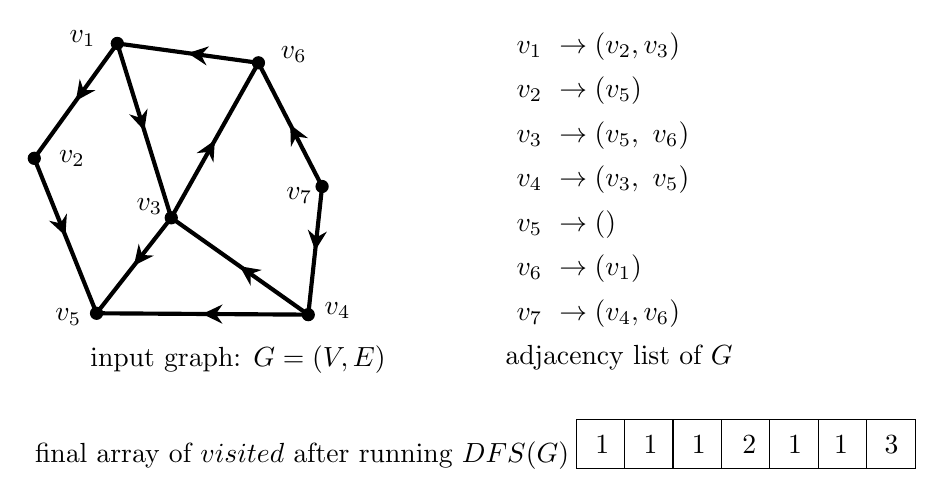
\begin{tikzpicture}[x=0.5pt,y=0.5pt,yscale=-1,xscale=1]
%uncomment if require: \path (0,342); %set diagram left start at 0, and has height of 342

%Flowchart: Connector [id:dp9968125919431555] 
\draw  [fill={rgb, 255:red, 0; green, 0; blue, 0 }  ,fill opacity=1 ] (78,14) .. controls (78,11.58) and (79.96,9.62) .. (82.38,9.62) .. controls (84.79,9.62) and (86.75,11.58) .. (86.75,14) .. controls (86.75,16.42) and (84.79,18.38) .. (82.38,18.38) .. controls (79.96,18.38) and (78,16.42) .. (78,14) -- cycle ;
%Flowchart: Connector [id:dp31888007270335605] 
\draw  [fill={rgb, 255:red, 0; green, 0; blue, 0 }  ,fill opacity=1 ] (180,28) .. controls (180,25.58) and (181.96,23.62) .. (184.38,23.62) .. controls (186.79,23.62) and (188.75,25.58) .. (188.75,28) .. controls (188.75,30.42) and (186.79,32.38) .. (184.38,32.38) .. controls (181.96,32.38) and (180,30.42) .. (180,28) -- cycle ;
%Flowchart: Connector [id:dp7333018163719219] 
\draw  [fill={rgb, 255:red, 0; green, 0; blue, 0 }  ,fill opacity=1 ] (63,209) .. controls (63,206.58) and (64.96,204.62) .. (67.38,204.62) .. controls (69.79,204.62) and (71.75,206.58) .. (71.75,209) .. controls (71.75,211.42) and (69.79,213.38) .. (67.38,213.38) .. controls (64.96,213.38) and (63,211.42) .. (63,209) -- cycle ;
%Flowchart: Connector [id:dp3353783499113435] 
\draw  [fill={rgb, 255:red, 0; green, 0; blue, 0 }  ,fill opacity=1 ] (18,97) .. controls (18,94.58) and (19.96,92.62) .. (22.38,92.62) .. controls (24.79,92.62) and (26.75,94.58) .. (26.75,97) .. controls (26.75,99.42) and (24.79,101.38) .. (22.38,101.38) .. controls (19.96,101.38) and (18,99.42) .. (18,97) -- cycle ;
%Flowchart: Connector [id:dp041293046821785806] 
\draw  [fill={rgb, 255:red, 0; green, 0; blue, 0 }  ,fill opacity=1 ] (117,140) .. controls (117,137.58) and (118.96,135.62) .. (121.38,135.62) .. controls (123.79,135.62) and (125.75,137.58) .. (125.75,140) .. controls (125.75,142.42) and (123.79,144.38) .. (121.38,144.38) .. controls (118.96,144.38) and (117,142.42) .. (117,140) -- cycle ;
%Straight Lines [id:da670830947000866] 
\draw [color={rgb, 255:red, 0; green, 0; blue, 0 }  ,draw opacity=1 ][line width=1.5]    (22.38,97) -- (82.38,14) ;
\draw [shift={(52.38,55.5)}, rotate = 305.86] [fill={rgb, 255:red, 0; green, 0; blue, 0 }  ,fill opacity=1 ][line width=0.08]  [draw opacity=0] (14.56,-6.99) -- (0,0) -- (14.56,6.99) -- (9.67,0) -- cycle    ;
%Straight Lines [id:da11972331039419015] 
\draw [color={rgb, 255:red, 0; green, 0; blue, 0 }  ,draw opacity=1 ][line width=1.5]    (67.38,209) -- (121.38,140) ;
\draw [shift={(94.38,174.5)}, rotate = 308.05] [fill={rgb, 255:red, 0; green, 0; blue, 0 }  ,fill opacity=1 ][line width=0.08]  [draw opacity=0] (14.56,-6.99) -- (0,0) -- (14.56,6.99) -- (9.67,0) -- cycle    ;
%Straight Lines [id:da5479420807598677] 
\draw [color={rgb, 255:red, 0; green, 0; blue, 0 }  ,draw opacity=1 ][line width=1.5]    (121.38,140) -- (82.38,14) ;
\draw [shift={(101.88,77)}, rotate = 252.8] [fill={rgb, 255:red, 0; green, 0; blue, 0 }  ,fill opacity=1 ][line width=0.08]  [draw opacity=0] (14.56,-6.99) -- (0,0) -- (14.56,6.99) -- (9.67,0) -- cycle    ;
%Straight Lines [id:da5035840510752034] 
\draw [color={rgb, 255:red, 0; green, 0; blue, 0 }  ,draw opacity=1 ][line width=1.5]    (67.38,209) -- (22.38,97) ;
\draw [shift={(44.88,153)}, rotate = 248.11] [fill={rgb, 255:red, 0; green, 0; blue, 0 }  ,fill opacity=1 ][line width=0.08]  [draw opacity=0] (14.56,-6.99) -- (0,0) -- (14.56,6.99) -- (9.67,0) -- cycle    ;
%Flowchart: Connector [id:dp2827777113276231] 
\draw  [fill={rgb, 255:red, 0; green, 0; blue, 0 }  ,fill opacity=1 ] (216,210) .. controls (216,207.58) and (217.96,205.62) .. (220.38,205.62) .. controls (222.79,205.62) and (224.75,207.58) .. (224.75,210) .. controls (224.75,212.42) and (222.79,214.38) .. (220.38,214.38) .. controls (217.96,214.38) and (216,212.42) .. (216,210) -- cycle ;
%Straight Lines [id:da4794154088615755] 
\draw [color={rgb, 255:red, 0; green, 0; blue, 0 }  ,draw opacity=1 ][line width=1.5]    (220.38,210) -- (121.38,140) ;
\draw [shift={(170.88,175)}, rotate = 35.26] [fill={rgb, 255:red, 0; green, 0; blue, 0 }  ,fill opacity=1 ][line width=0.08]  [draw opacity=0] (14.56,-6.99) -- (0,0) -- (14.56,6.99) -- (9.67,0) -- cycle    ;
%Straight Lines [id:da5289435706939755] 
\draw [color={rgb, 255:red, 0; green, 0; blue, 0 }  ,draw opacity=1 ][line width=1.5]    (67.38,209) -- (220.38,210) ;
\draw [shift={(143.88,209.5)}, rotate = 0.37] [fill={rgb, 255:red, 0; green, 0; blue, 0 }  ,fill opacity=1 ][line width=0.08]  [draw opacity=0] (14.56,-6.99) -- (0,0) -- (14.56,6.99) -- (9.67,0) -- cycle    ;
%Flowchart: Connector [id:dp11045273073359585] 
\draw  [fill={rgb, 255:red, 0; green, 0; blue, 0 }  ,fill opacity=1 ] (226,117.38) .. controls (226,114.96) and (227.96,113) .. (230.38,113) .. controls (232.79,113) and (234.75,114.96) .. (234.75,117.38) .. controls (234.75,119.79) and (232.79,121.75) .. (230.38,121.75) .. controls (227.96,121.75) and (226,119.79) .. (226,117.38) -- cycle ;
%Straight Lines [id:da34875485243986093] 
\draw [color={rgb, 255:red, 0; green, 0; blue, 0 }  ,draw opacity=1 ][line width=1.5]    (230.38,117.38) -- (184.38,28) ;
\draw [shift={(207.38,72.69)}, rotate = 62.77] [fill={rgb, 255:red, 0; green, 0; blue, 0 }  ,fill opacity=1 ][line width=0.08]  [draw opacity=0] (14.56,-6.99) -- (0,0) -- (14.56,6.99) -- (9.67,0) -- cycle    ;
%Shape: Grid [id:dp773013244810068] 
\draw  [draw opacity=0] (414,285.87) -- (659,285.87) -- (659,320.87) -- (414,320.87) -- cycle ; \draw   (449,285.87) -- (449,320.87)(484,285.87) -- (484,320.87)(519,285.87) -- (519,320.87)(554,285.87) -- (554,320.87)(589,285.87) -- (589,320.87)(624,285.87) -- (624,320.87) ; \draw    ; \draw   (414,285.87) -- (659,285.87) -- (659,320.87) -- (414,320.87) -- cycle ;
%Straight Lines [id:da6438487476256122] 
\draw [color={rgb, 255:red, 0; green, 0; blue, 0 }  ,draw opacity=1 ][line width=1.5]    (121.38,140) -- (184.38,28) ;
\draw [shift={(152.88,84)}, rotate = 119.36] [fill={rgb, 255:red, 0; green, 0; blue, 0 }  ,fill opacity=1 ][line width=0.08]  [draw opacity=0] (14.56,-6.99) -- (0,0) -- (14.56,6.99) -- (9.67,0) -- cycle    ;
%Straight Lines [id:da22153267574847257] 
\draw [color={rgb, 255:red, 0; green, 0; blue, 0 }  ,draw opacity=1 ][line width=1.5]    (82.38,14) -- (184.38,28) ;
\draw [shift={(133.38,21)}, rotate = 7.82] [fill={rgb, 255:red, 0; green, 0; blue, 0 }  ,fill opacity=1 ][line width=0.08]  [draw opacity=0] (14.56,-6.99) -- (0,0) -- (14.56,6.99) -- (9.67,0) -- cycle    ;
%Straight Lines [id:da1089086337589269] 
\draw [color={rgb, 255:red, 0; green, 0; blue, 0 }  ,draw opacity=1 ][line width=1.5]    (220.38,210) -- (230.38,117.38) ;
\draw [shift={(225.38,163.69)}, rotate = 276.16] [fill={rgb, 255:red, 0; green, 0; blue, 0 }  ,fill opacity=1 ][line width=0.08]  [draw opacity=0] (14.56,-6.99) -- (0,0) -- (14.56,6.99) -- (9.67,0) -- cycle    ;

% Text Node
\draw (46,3) node [anchor=north west][inner sep=0.75pt]   [align=left] {$\displaystyle v_{1}$};
% Text Node
\draw (94.38,124.38) node [anchor=north west][inner sep=0.75pt]   [align=left] {$\displaystyle v_{3}$};
% Text Node
\draw (35.75,204) node [anchor=north west][inner sep=0.75pt]   [align=left] {$\displaystyle v_{5}$};
% Text Node
\draw (230.38,199.38) node [anchor=north west][inner sep=0.75pt]   [align=left] {$\displaystyle v_{4}$};
% Text Node
\draw (38.38,89.38) node [anchor=north west][inner sep=0.75pt]   [align=left] {$\displaystyle v_{2}$};
% Text Node
\draw (369,4.09) node [anchor=north west][inner sep=0.75pt]   [align=left] {$\displaystyle v_{1} \ \rightarrow ( v_{2} ,v_{3})$};
% Text Node
\draw (369,36.26) node [anchor=north west][inner sep=0.75pt]   [align=left] {$\displaystyle v_{2} \ \rightarrow ( v_{5})$};
% Text Node
\draw (369,68.43) node [anchor=north west][inner sep=0.75pt]   [align=left] {$\displaystyle v_{3} \ \rightarrow ( v_{5} ,\ v_{6})$};
% Text Node
\draw (369,100.6) node [anchor=north west][inner sep=0.75pt]   [align=left] {$\displaystyle v_{4} \ \rightarrow ( v_{3} ,\ v_{5})$ \ };
% Text Node
\draw (369,132.77) node [anchor=north west][inner sep=0.75pt]   [align=left] {$\displaystyle v_{5} \ \rightarrow ()$};
% Text Node
\draw (198.75,14.35) node [anchor=north west][inner sep=0.75pt]   [align=left] {$\displaystyle v_{6}$};
% Text Node
\draw (202.75,116.35) node [anchor=north west][inner sep=0.75pt]   [align=left] {$\displaystyle v_{7}$};
% Text Node
\draw (369,164.94) node [anchor=north west][inner sep=0.75pt]   [align=left] {$\displaystyle v_{6} \ \rightarrow ( v_{1} )$ \ };
% Text Node
\draw (369,197.09) node [anchor=north west][inner sep=0.75pt]   [align=left] {$\displaystyle v_{7} \ \rightarrow ( v_{4} ,v_{6})$};
% Text Node
\draw (61,230.93) node [anchor=north west][inner sep=0.75pt]   [align=left] {input graph: $\displaystyle G=( V,E)$};
% Text Node
\draw (361,229.93) node [anchor=north west][inner sep=0.75pt]   [align=left] {adjacency list of $\displaystyle G$};
% Text Node
\draw (21,299.93) node [anchor=north west][inner sep=0.75pt]   [align=left] {final array of $\displaystyle visited$ after running $\displaystyle DFS( G)$};
% Text Node
\draw (426,295.37) node [anchor=north west][inner sep=0.75pt]   [align=left] {$\displaystyle 1$};
% Text Node
\draw (460.83,295.37) node [anchor=north west][inner sep=0.75pt]   [align=left] {$\displaystyle 1$};
% Text Node
\draw (495.66,295.37) node [anchor=north west][inner sep=0.75pt]   [align=left] {$\displaystyle 1$};
% Text Node
\draw (598.49,295.37) node [anchor=north west][inner sep=0.75pt]   [align=left] {$\displaystyle 1$};
% Text Node
\draw (565.32,295.37) node [anchor=north west][inner sep=0.75pt]   [align=left] {$\displaystyle 1$};
% Text Node
\draw (532.15,295.37) node [anchor=north west][inner sep=0.75pt]   [align=left] {$\displaystyle 2$};
% Text Node
\draw (635,295.37) node [anchor=north west][inner sep=0.75pt]   [align=left] {$\displaystyle 3$};


\end{tikzpicture}

}
\caption{Example of running DFS~(with timing) on a directed graph. 
The $[pre,post]$ interval for each vertex
is marked next to each vertex. The $postlist$ for this run is $postlist = (v_5,v_2,v_6,v_3,v_1,v_7,v_4)$.}
\end{figure}
